\usepgflibrary{shapes.misc}
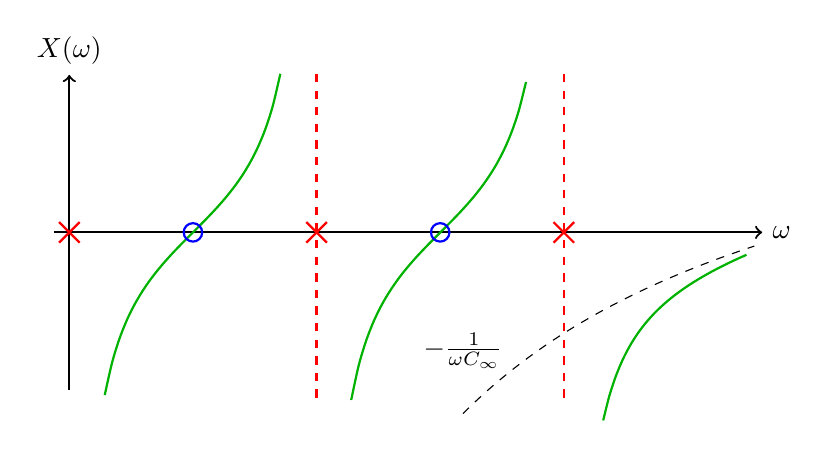
\begin{tikzpicture}[smooth]
% Achsen
\draw[->, thick] (-0.2,0) -- +(9,0) node[right] {$\omega$}; % Horizontal
\draw[->, thick] (0,-2) -- +(0,4) node[above] {$X(\omega)$}; % Vertikal

% Plots
\draw[color=green!70!black, thick] plot[domain=0.45:2.68] (\x,{tan((\x -1.57) r)}); % Erster Tan
\draw[color=green!70!black, thick] plot[domain=3.58:5.8] (\x,{tan((\x -1.57) r)}); % zweiter Tan
\draw[color=green!70!black, thick] plot[domain=6.78:8.6] (\x,{ ((0.25 * \x) -1/(\x -6.3)) -2 }); % letzte kurve

% Poolstellen
\draw[dashed, thick, draw=red] (3.14,-2.1) -- +(0,4.2); % Poolstelle 1
\draw[dashed, thick, draw=red] (6.28,-2.1) -- +(0,4.2); % Poolstelle 2
\node[cross out, draw=red, thick] (wr1) at (3.14,0) {};
\node[cross out, draw=red, thick] at (6.28,0) {};
\node[cross out, draw=red, thick] at (0,0) {};


\draw[dashed] plot[domain=5:8.7] (\x, { (-1 /(0.04 * \x)) + 2.7 });
\node (wL) at (5,-1.5) {$- \frac{1}{\omega C_\infty}$};

% Nullstellen
\node[rounded rectangle, draw=blue, thick] at(1.57,0) {};
\node[rounded rectangle, draw=blue, thick] at(4.71,0) {};
\end{tikzpicture}